\chapter{Experimental Setting}

The current chapter is divided into two sections. In the first one we will describe the benchmark of the experiment regarding the creation of the RL agent and its results. In the second one we will describe the same experiment applied to humans and its results.

\section{Benchmark}

\paragraph{Test Functions}

As already explained, the experiment described in this work is about maximize black-box functions adopting an RL based approach. The first important choice is about selecting suitable \textit{test functions}. In applied mathematics, test functions, also known as \textit{artificial landscapes}, are useful to evaluate characteristics of optimization algorithms. We have chosen four test functions for this work:

\begin{itemize}
	\item Himmelblau' s Function;
	\item Paraboloid of Revolution;
	\item Beale Function;
	\item Styblinski-Tang' s Revised Function.	
\end{itemize}

\subparagraph{Himmelblau' s Function} In mathematical optimization, Himmelblau' s function is a continuous, bivariate, multi-modal function introduced by David Mautner Himmelblau (1924–2011). The original function is defined by: 

\begin{equation}
	f(x, y) = (x^2 + y -11)^2 + (x + y^2 - 7)^2
\end{equation}

\begin{figure}[h!]
	\centering
	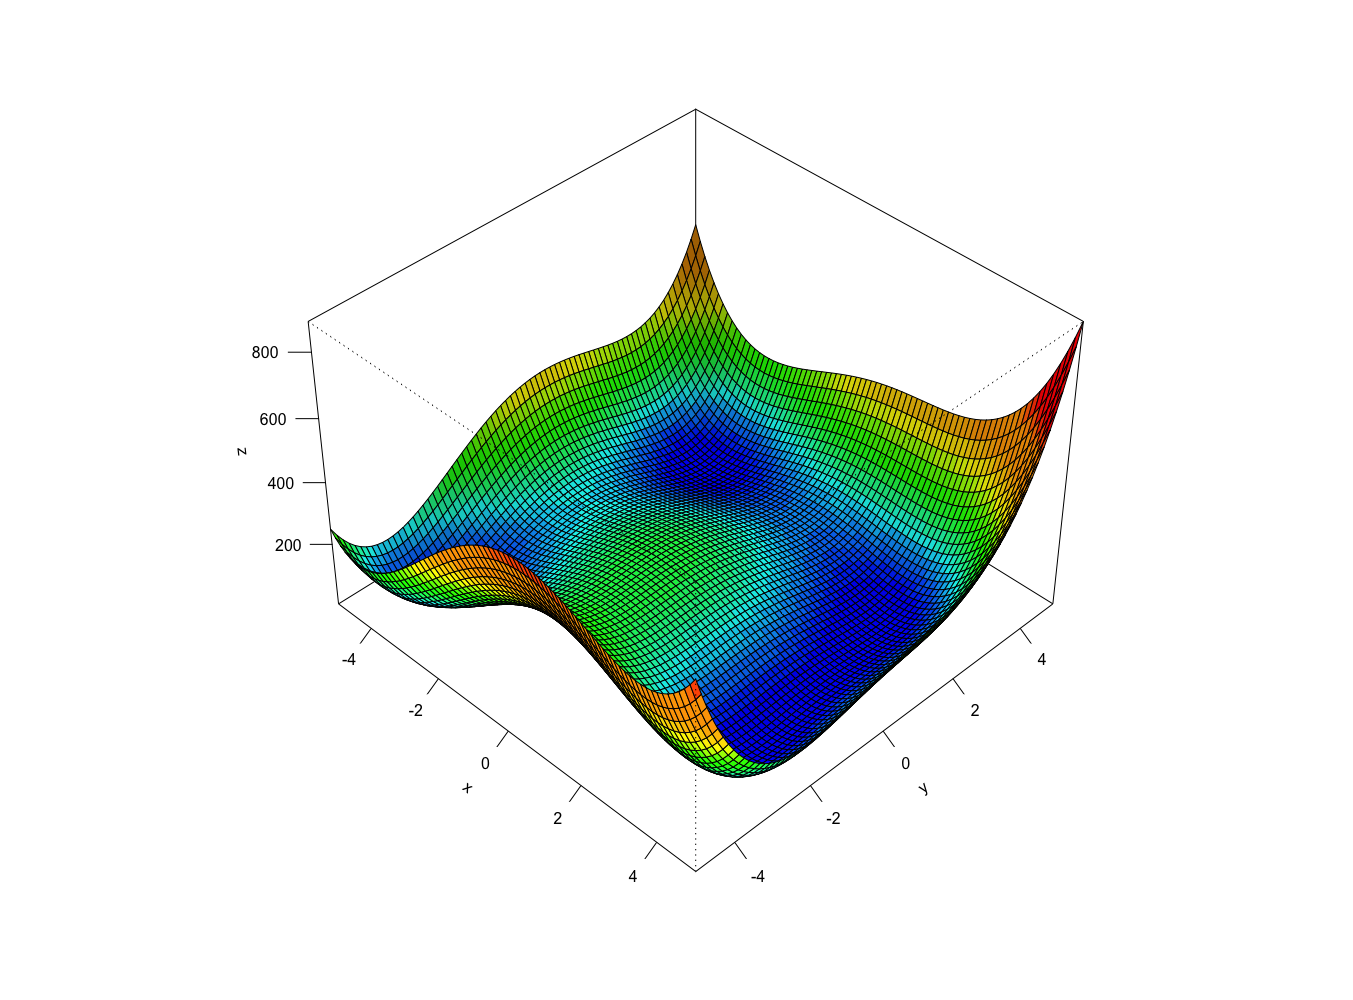
\includegraphics[width= 14cm, height = 14cm]{originalHimmelblau.png}
	\caption{Original Himmelblau' s Function.}
	\label{fig:OriginalHimmelblauFunction}
\end{figure}

It has four local minima :

\begin{itemize}
	\item $f(3.0, 2.0) = 0.0$;
	\item $f(-2.805118, 3.131312) = 0.0$;
	\item $f(-3.779310, -3.283186) = 0.0$;
	\item $f(3.584428, -1848126) = 0.0$.
\end{itemize}
	
The function can be defined on any input domain but it is usually evaluated on $x \in [-5, 5]$ and $y \in [-5, 5]$.

\begin{figure}[h!]
	\centering
	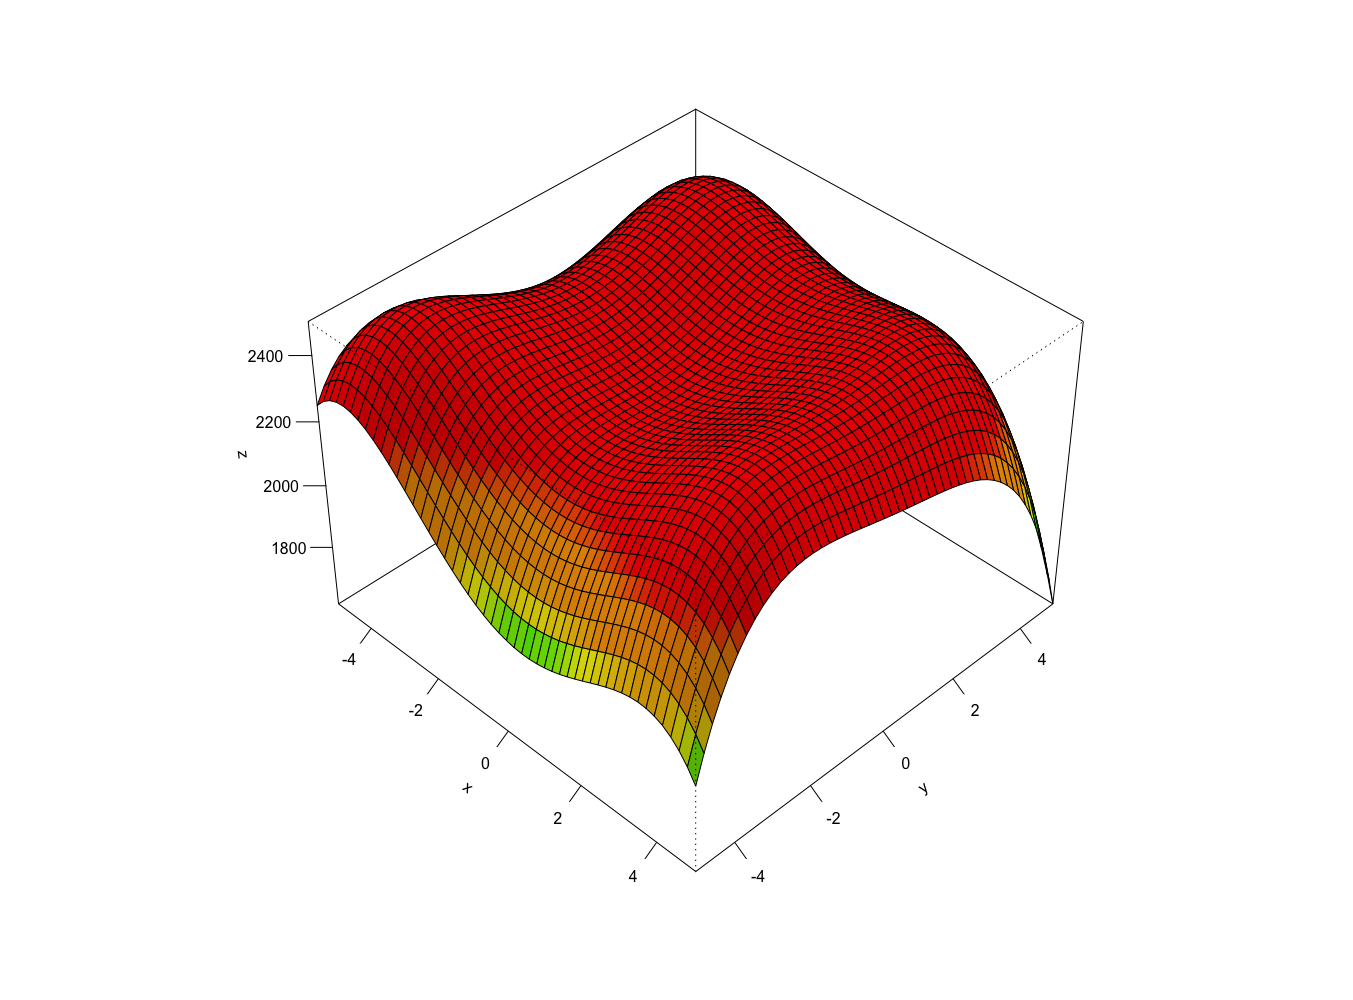
\includegraphics[width= 14cm, height = 14cm]{modifiedHimmelblau.png}
	\caption{Customized Himmelblau' s Function.}
	\label{fig:CustomizedHimmelblauFunction}
\end{figure}

Because of our aim to maximize we inverted the function as follow :

\begin{equation}
f(x, y) = -(x^2 + y -11)^2 + (x + y^2 - 7)^2
\end{equation}

and we picked it up of $2500$ units in order to have as less as possible negative values. So the final adopted function is :
 
\begin{equation}
f(x, y) = -(x^2 + y -11)^2 + (x + y^2 - 7)^2 + 2500
\end{equation}

This function has its global maximum in $f(x, y) = 2500$. \\

In order to represent this customized version of Himmelblau' s Function using Java Graphical Environment, we mapped it in a space of $600 \times 600$ pixels and we properly rotated it. The resulting contour plot is the one represented in figure ~\ref{fig:ContourPlotCustomizedHimmelblauFunction}. \\

\begin{figure}[h!]
	\centering
	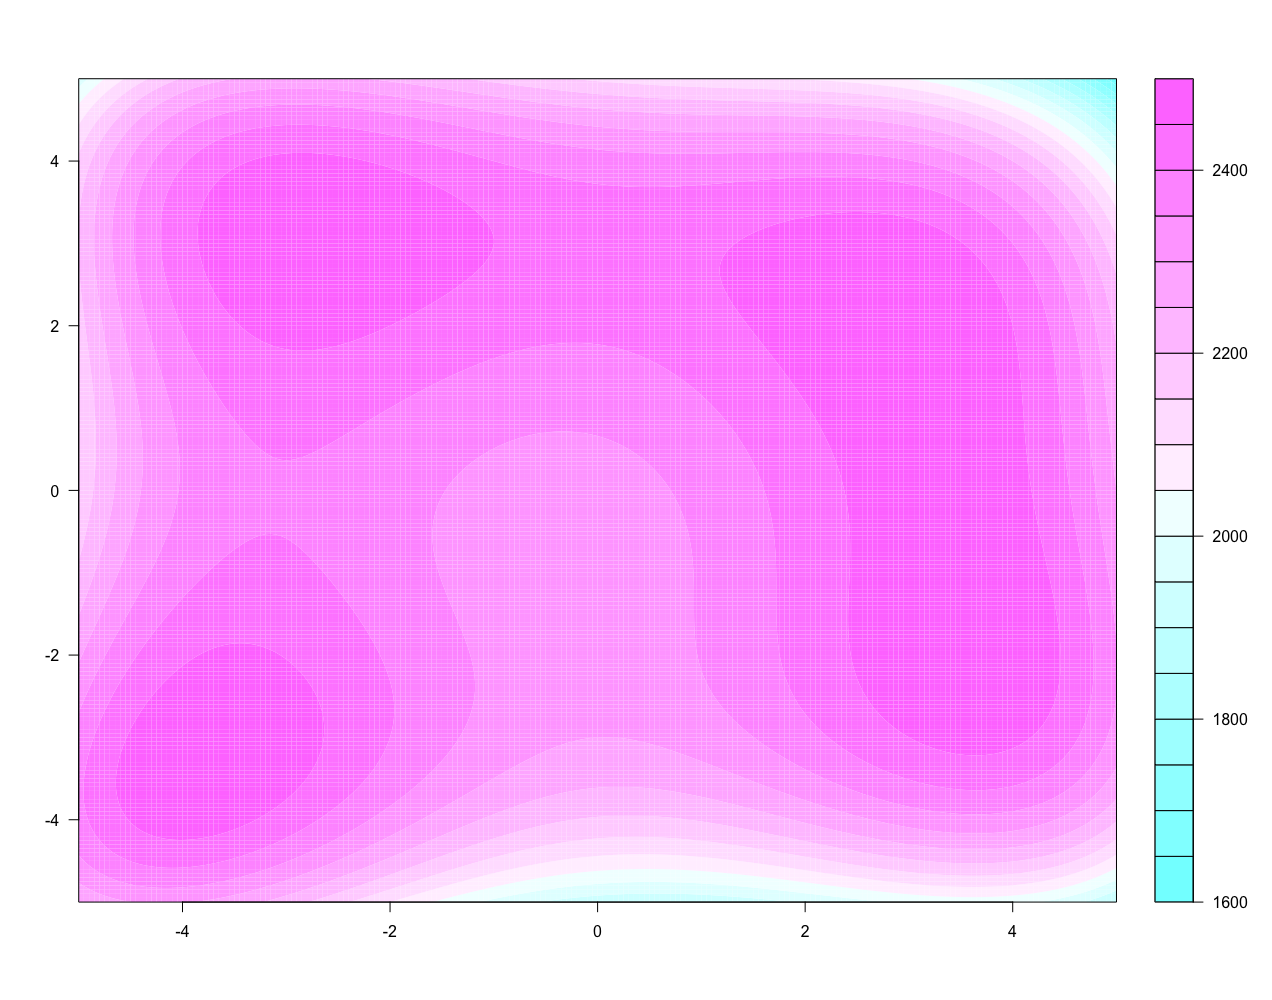
\includegraphics[width= 9cm, height = 9cm]{himmelblau.png}
	\caption{Contour plot of customized version of Himmelblau' s Function.}
	\label{fig:ContourPlotCustomizedHimmelblauFunction}
\end{figure}
 
\subparagraph{Paraboloid of Revolution} In mathematical optimization, Paraboloid of Revolution is a continuous, bivariate, multi-modal function. \\

The original function is defined by: 

\begin{equation}
f(x, y) = (x^2 + y^2) 
\end{equation}

\begin{figure}[h!]
	\centering
	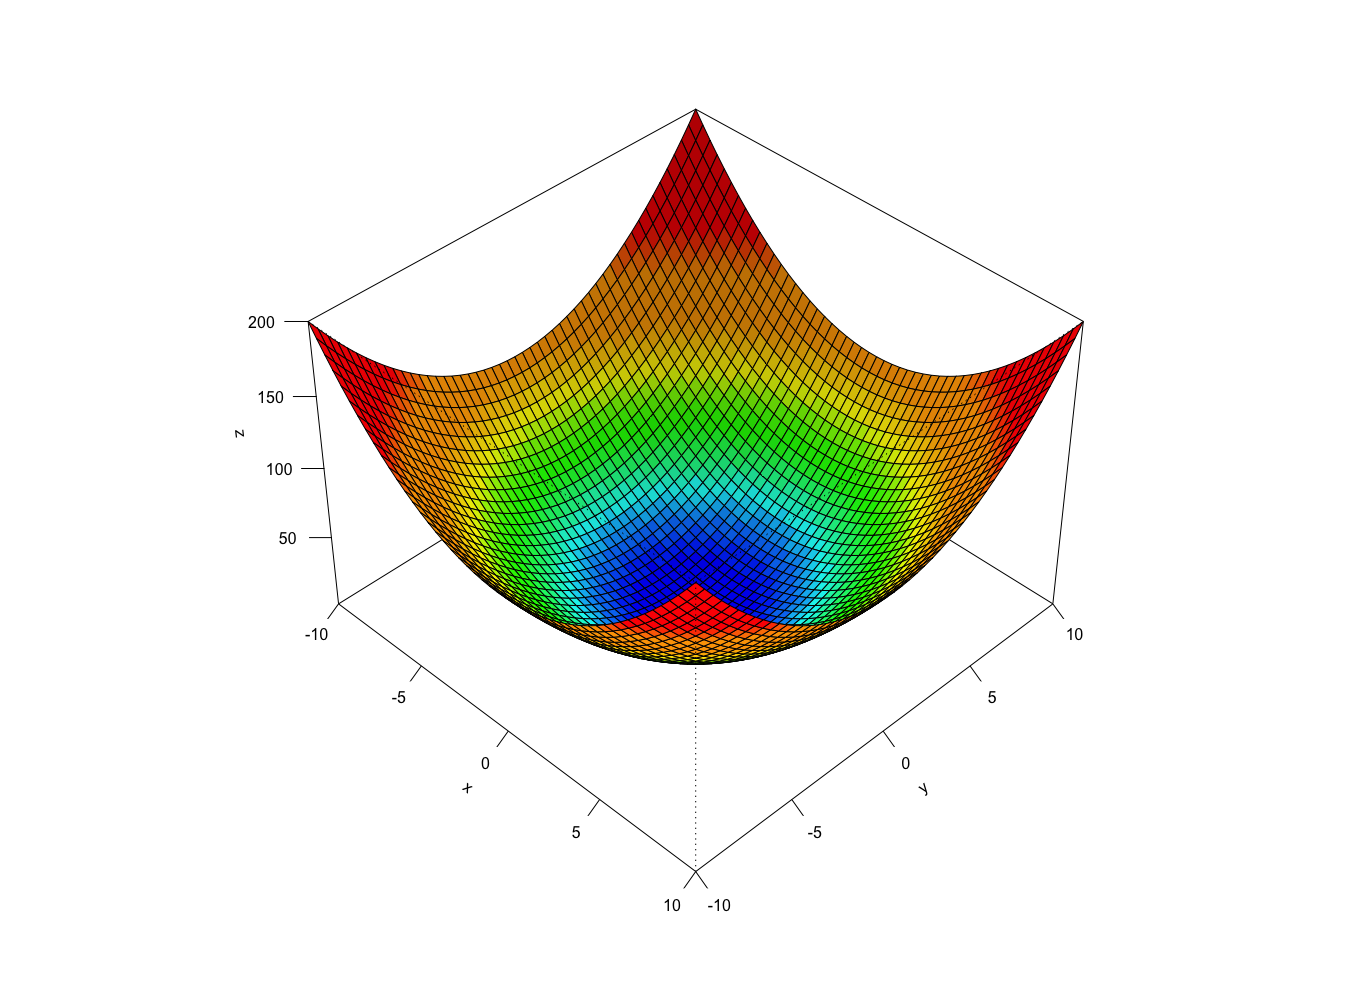
\includegraphics[width= 14cm, height = 14cm]{originalParaboloid.png}
	\caption{Original Paraboloid of Revolution.}
	\label{fig:OriginalParaboloidOfRevolution}
\end{figure}

It has a global minimum in $f(x, y) = 0$. \\

The function can be defined on any input domain but it is usually evaluated on $x \in [-10, 10]$ and $y \in [-10, 10]$. 

\pagebreak

\begin{figure}[h!]
	\centering
	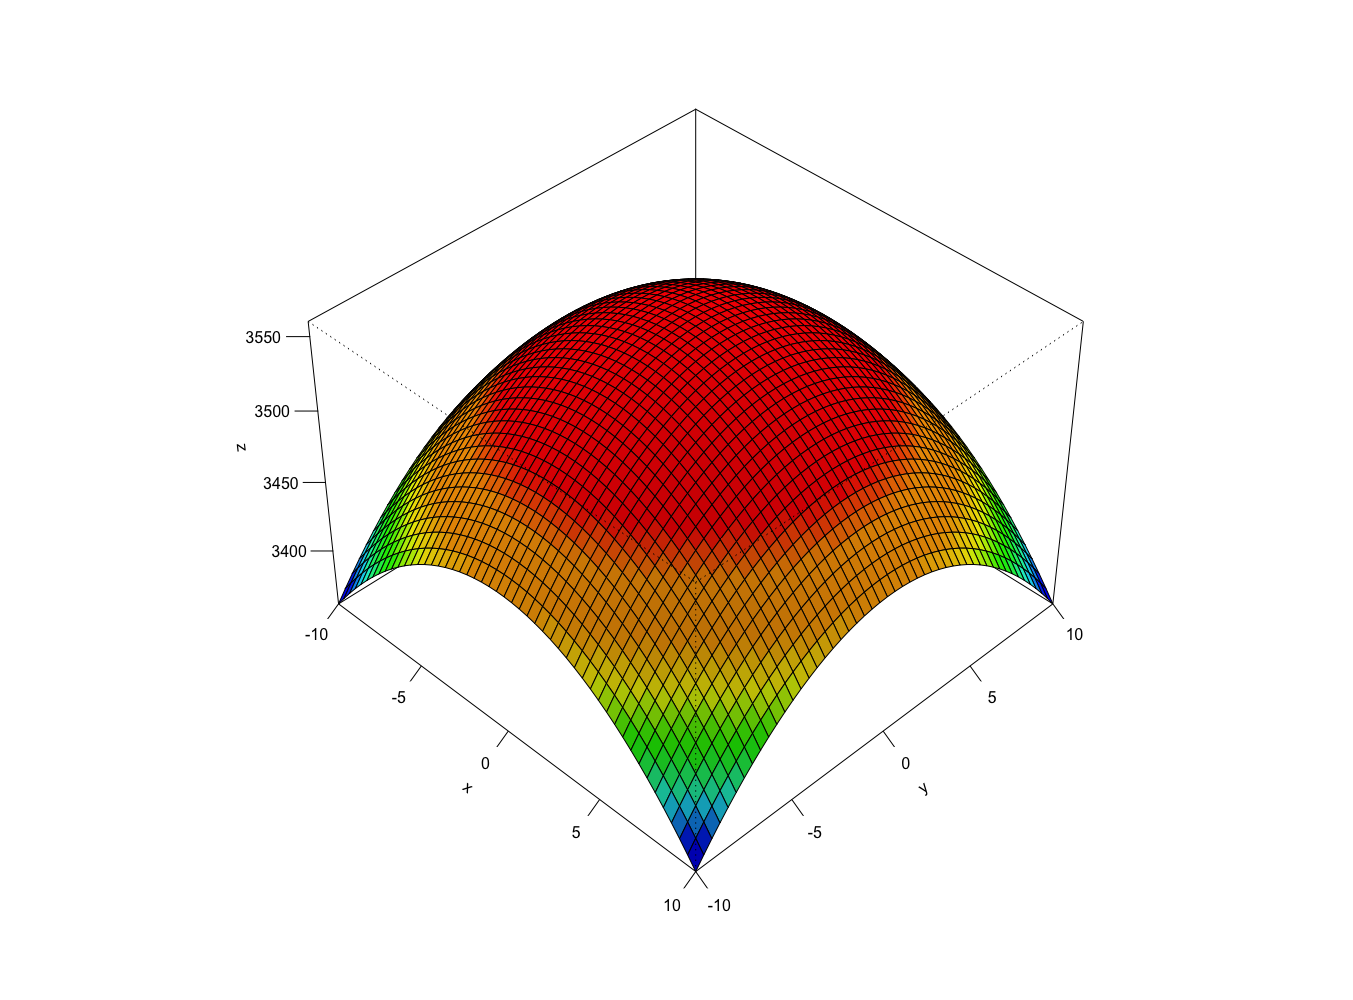
\includegraphics[width= 14cm, height = 14cm]{customizedParaboloid.png}
	\caption{Customized Paraboloid of Revolution.}
	\label{fig:CustomizedParaboloidOfRevolution}
\end{figure}

Because of our aim to maximize, we inverted the function as follow :

\begin{equation}
f(x, y) = -(x^2 + y^2)
\end{equation}

and we picked it up of $3560$ units in order to have as less as possible negative values. So the final adopted function is :

\begin{equation}
f(x, y) = -(x^2 + y^2) + 3560
\end{equation}

This function has its local maximum in $f(x, y) = 3560$.

In order to represent this customized version of Paraboloid of Revolution function using Java Graphical Environment, we mapped it in a space of $600 \times 600$ pixels and we properly rotated it. The resulting contour plot is the one represented in figure ~\ref{fig:ContourPlotCustomizedParabolicFunction} 

\begin{figure}[h!]
	\centering
	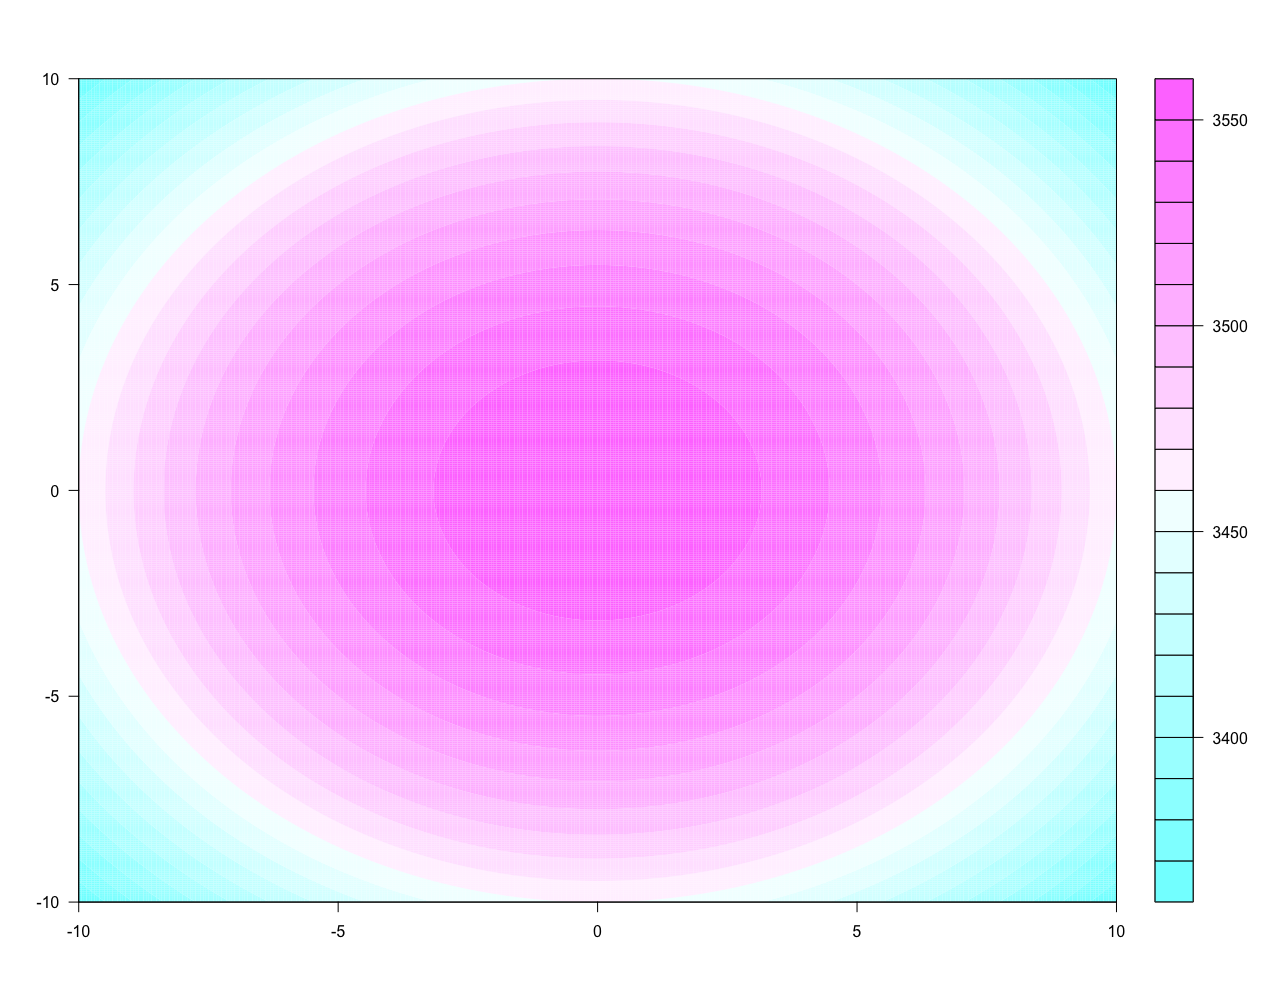
\includegraphics[width= 9cm, height = 9cm]{parabolic.png}
	\caption{Contour plot of customized Parabolic Function.}
	\label{fig:ContourPlotCustomizedParabolicFunction}
\end{figure}

\subparagraph{Beale Function} In mathematical optimization, Beale Function is a continuous, multi-modal function defined on a two-dimensional space. The function is defined by: 

\begin{equation}
f(x, y) = (1.5 - x + xy)^2 + (2.25 - x + xy^2)^2 + (2.625 - x + xy^3)^2
\end{equation}

\break

\begin{figure}[h!]
	\centering
	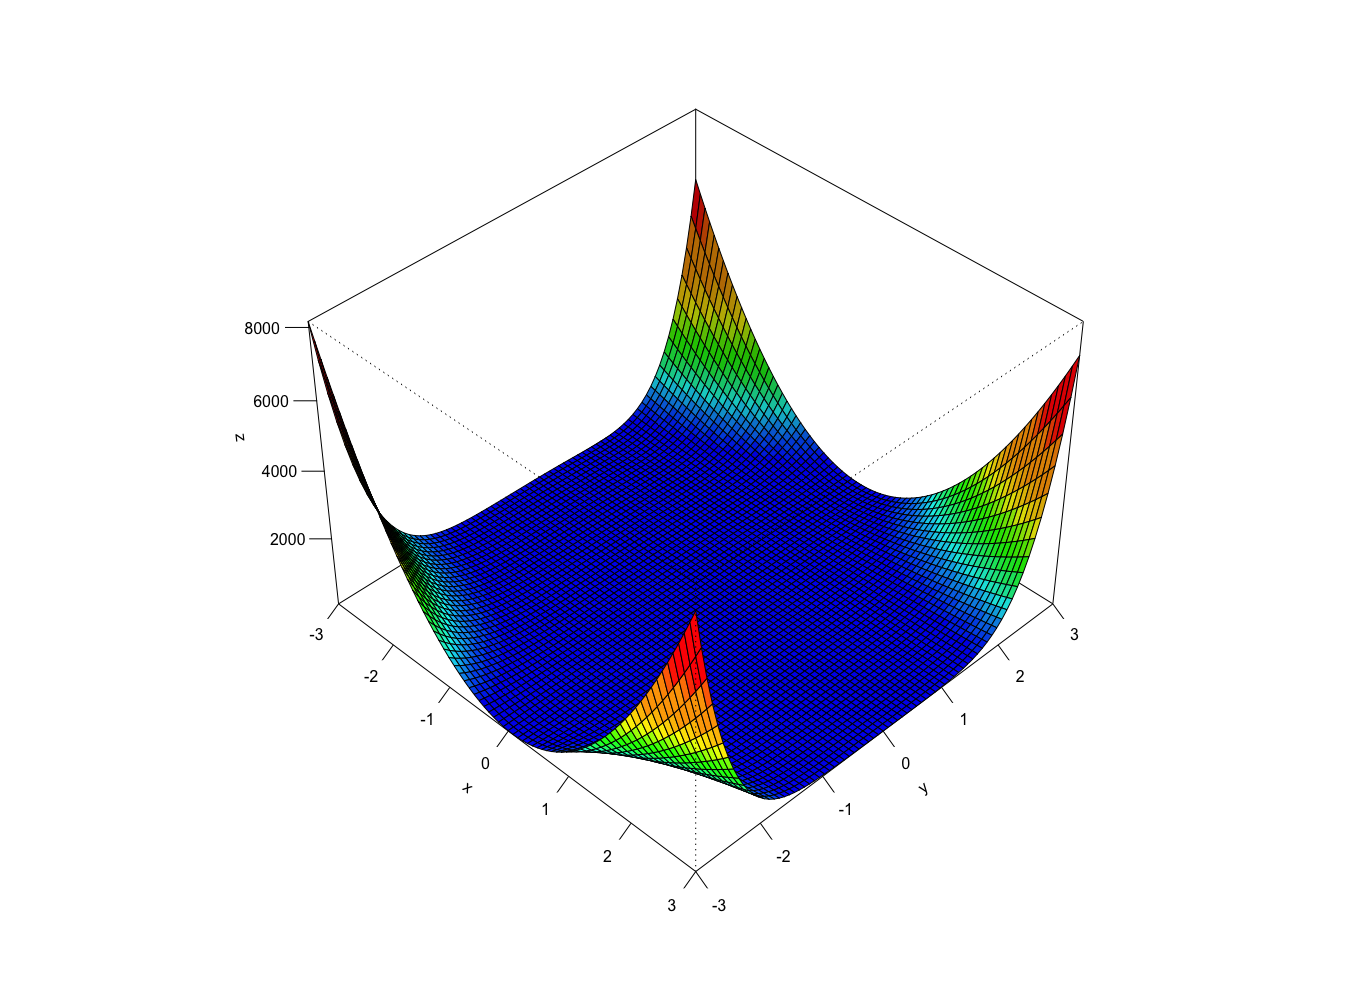
\includegraphics[width= 14cm, height = 14cm]{originalBeale.png}
	\caption{Original Beale Function.}
	\label{fig:OriginalBealeFunction}
\end{figure}

The function can be defined on any input domain but it is usually evaluated on $x \in [-3, 3]$ and $y \in [-3, 3]$. \\

It has one global minimum at: $f(x, y) = 0$. 

In this thesis our aim is to maximize. In order to do this we inverted the function as

\begin{equation}
f(x, y) = -((1.5 - x + xy)^2 + (2.25 - x + xy^2)^2 + (2.625 - x + xy^3)^2)
\end{equation}

\begin{figure}[h!]
	\centering
	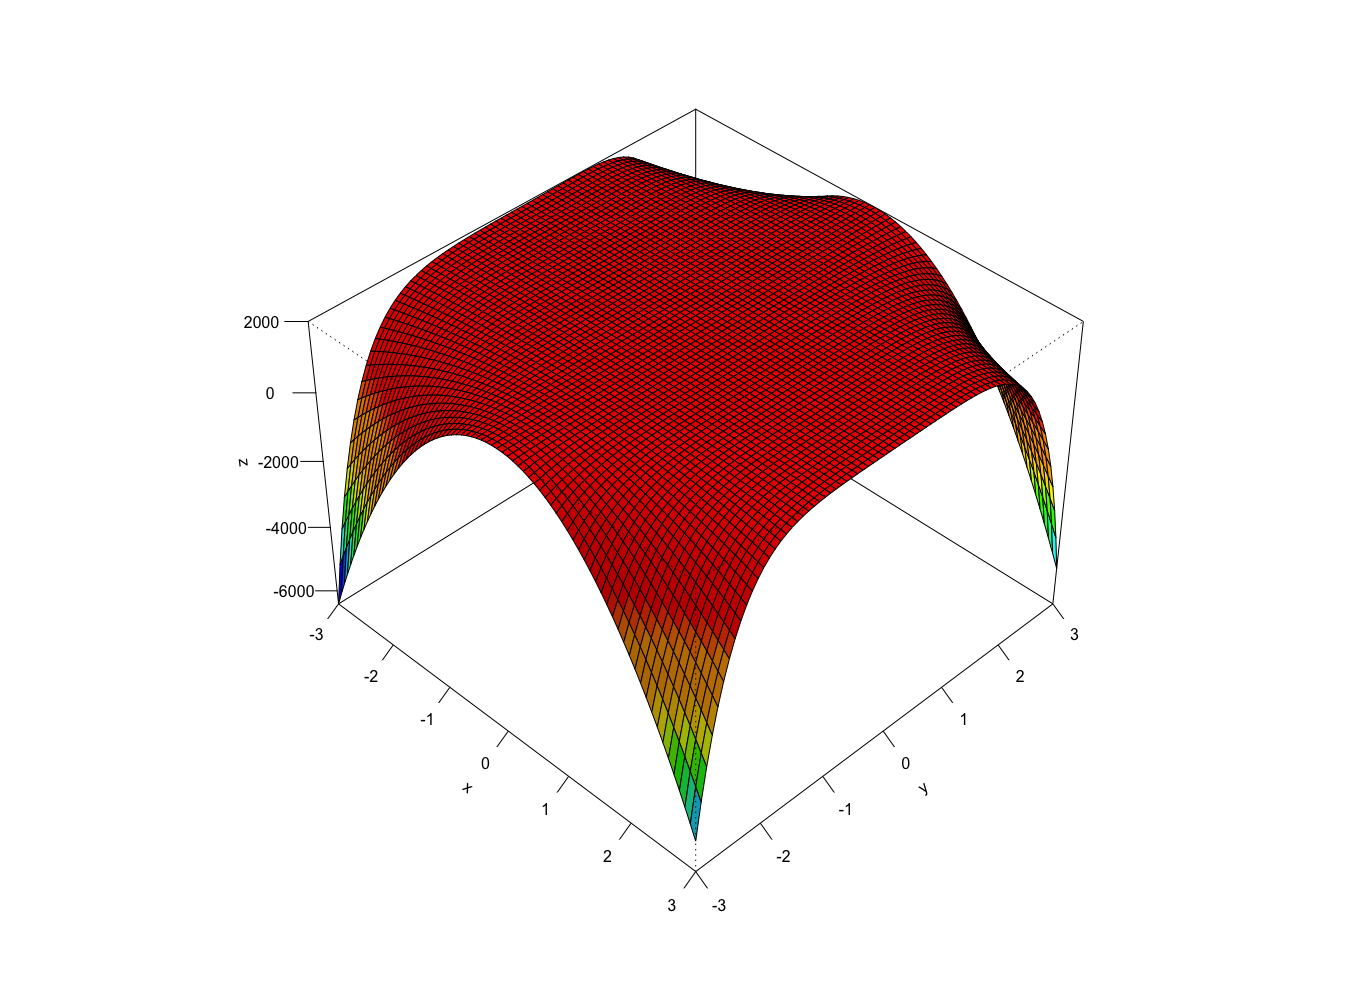
\includegraphics[width= 14cm, height = 14cm]{customizedBeale.png}
	\caption{Customized Beale Function.}
	\label{fig:CustomizedBealeFunction}
\end{figure}

and we picked it up of $2000$ units in order to have as less as possible negative values. So the final adopted function is :

\begin{equation}
f(x, y) = -((1.5 - x + xy)^2 + (2.25 - x + xy^2)^2 + (2.625 - x + xy^3)^2) + 2000
\end{equation}

This customized function has its global maximum in $f(x, y) = 1000$. \\

In order to represent this function using Java Graphical Environment we mapped it in a space of $600 \times 600$ pixels and we properly rotated it. The resulting contour plot is the one represented in figure ~\ref{fig:ContourPlotCustomizedBealeFunction} 

\begin{figure}[h!]
	\centering
	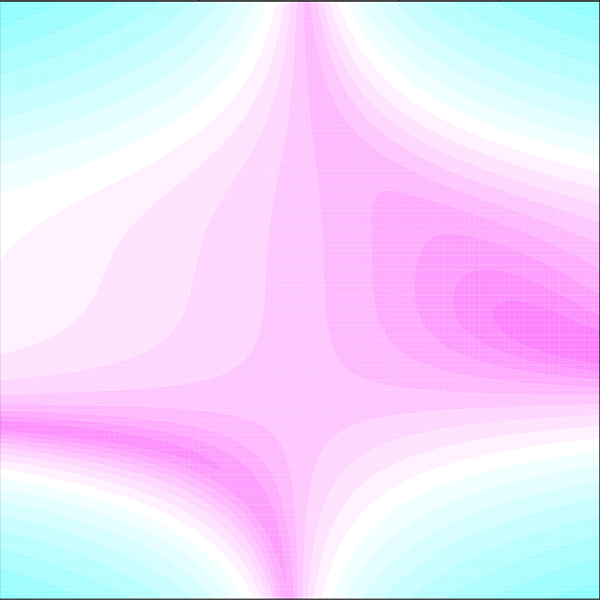
\includegraphics[width= 9cm, height = 9cm]{beale.png}
	\caption{Contour plot of customized Beale Function.}
	\label{fig:ContourPlotCustomizedBealeFunction}
\end{figure}

\subparagraph{Styblinski-Tang Revised Function} In mathematical optimization, Styblinski-Tang Function is a continuous, multi-modal function defined on a multi-dimensional space. The original function is defined by :

\begin{equation}
	f(x) = \dfrac{\sum_{i=1}^{n} x_{i}^4 -16x_{i}^2 +5x_{i}}{2}
\end{equation}

In this thesis we consider the bivariate version of the original function multiplied by two in order to make it less flattened :

\begin{equation}
f(x, y) = (x^4 - 16x^2 + 5x) + (y^4 - 16y^2 + 5y).
\end{equation}

\begin{figure}[h!]
	\centering
	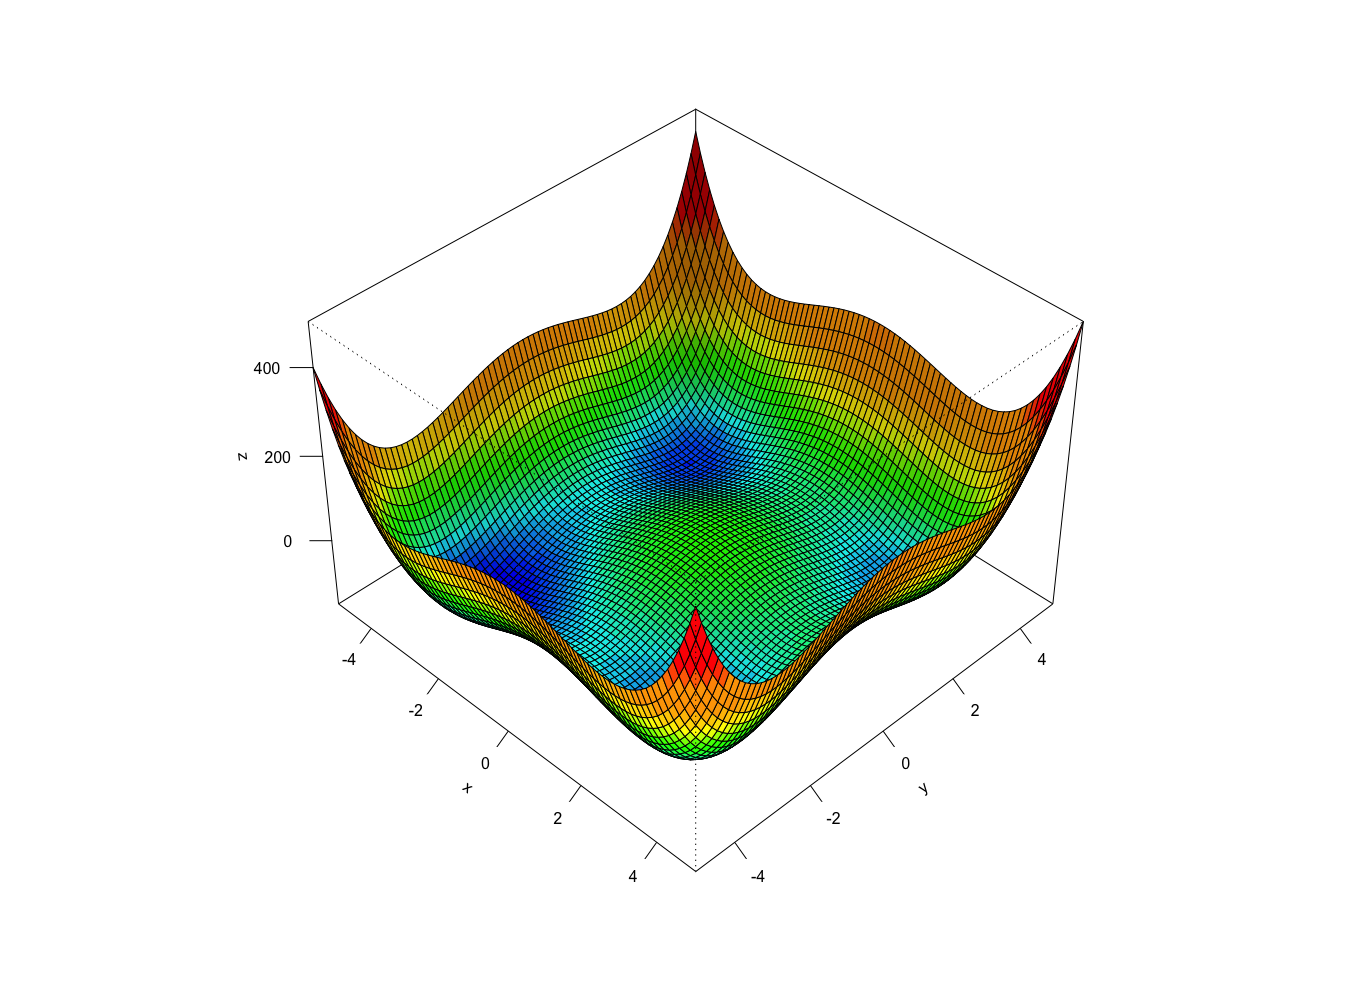
\includegraphics[width= 14cm, height = 14cm]{classicalStyblinski.png}
	\caption{Original Styblinski Function.}
	\label{fig:OriginalStyblinskiFunction}
\end{figure}

The function can be defined on any input domain but it is usually evaluated on $x \in [-5, 5]$ and $y \in [-5, 5]$. \\

In this thesis our aim is to maximize. In order to do this we inverted the function as

\begin{equation}
f(x, y) = -((x^4 - 16 * x^2 + 5 * x) + (y^4 - 16 * y^2 + 5 * y))
\end{equation}

\begin{figure}[h!]
	\centering
	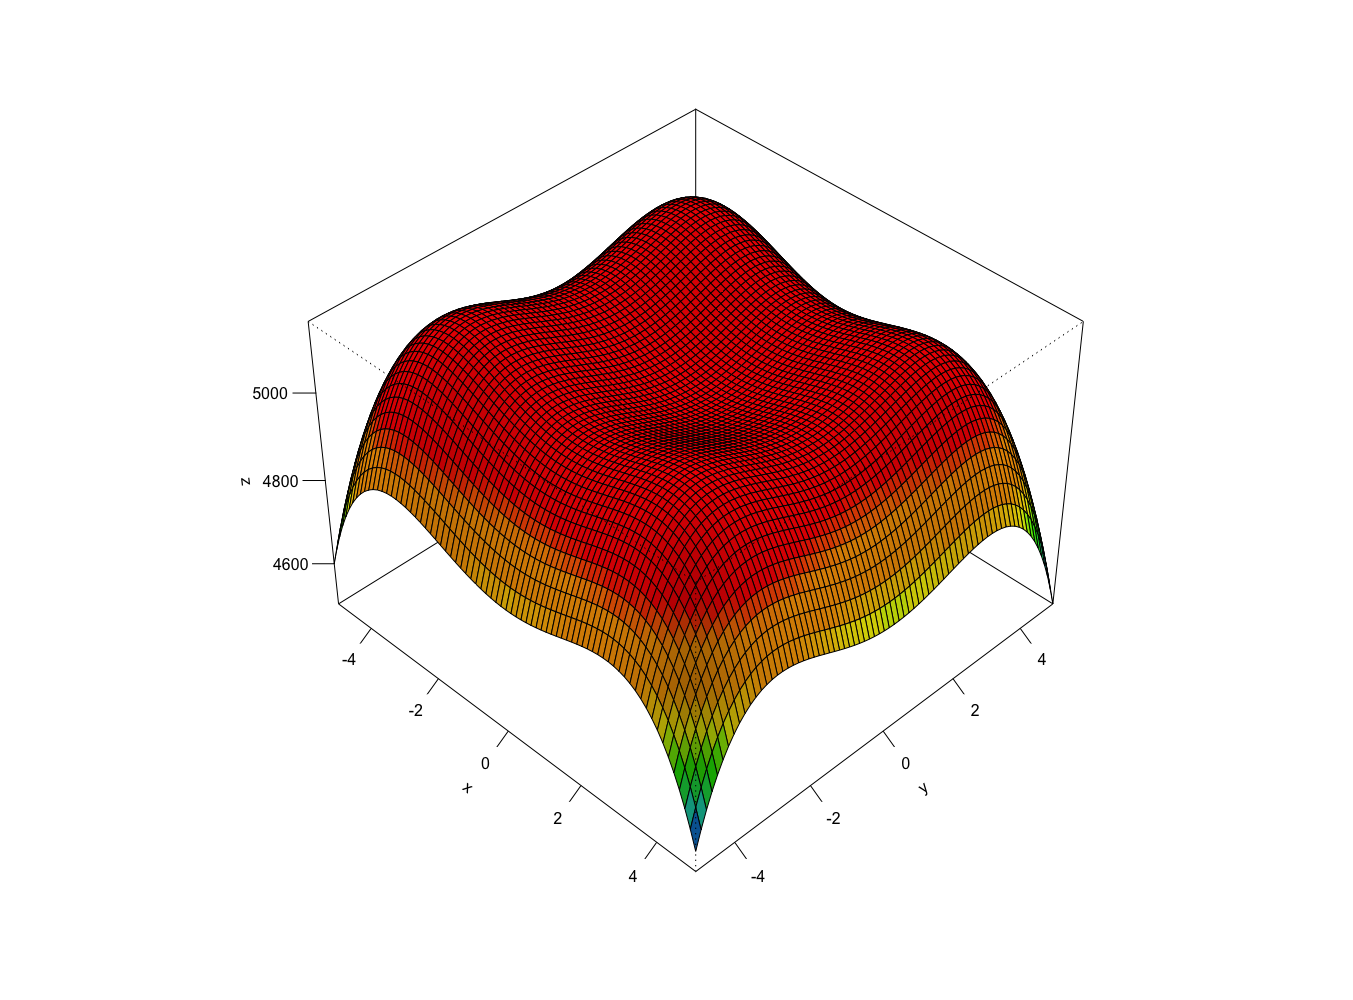
\includegraphics[width= 14cm, height = 14cm]{customizedStyblinski.png}
	\caption{Customized Styblinski Function.}
	\label{fig:CustomizedStyblinskiFunction}
\end{figure}

and we picked it up of $5000$ units in order to has as less as possible negative values. So the final adopted function is: 

\begin{equation}
f(x, y) = -((x^4 - 16 * x^2 + 5 * x) + (y^4 - 16 * y^2 + 5 * y)) + 5000
\end{equation}

This customized function has its global maximum in $f(x, y) = 5156.6638$. In order to represent this function using Java Graphical Environment we mapped its in a space of $600 \times 600$ pixels and we properly rotated its. The resulting contour plot is the one represented in figure ~\ref{fig:ContourStyblinskiFunction}.

\begin{figure}[h!]
	\centering
	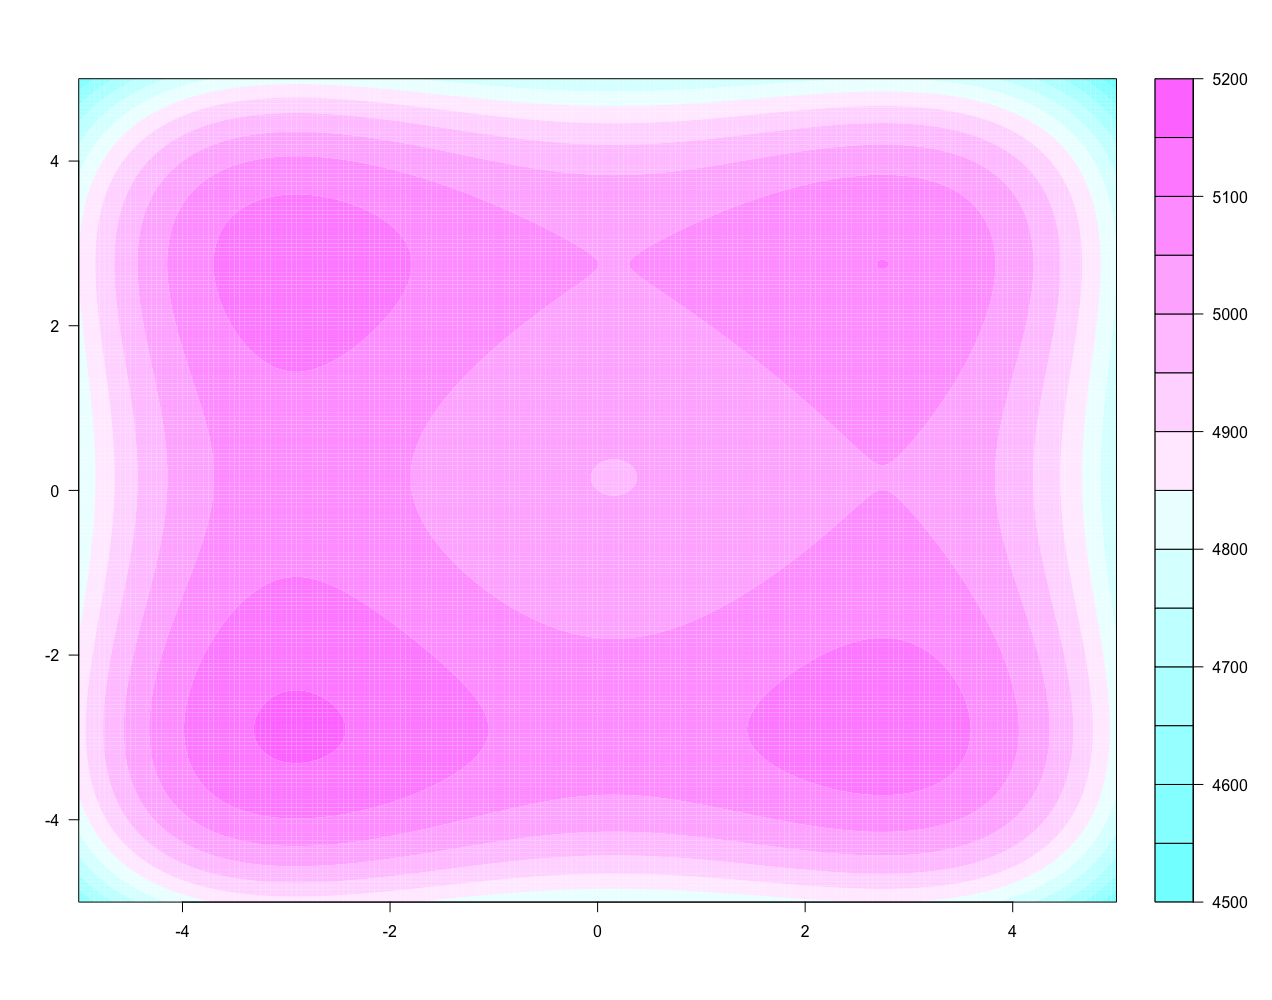
\includegraphics[width= 9cm, height = 9cm]{styblinski.png}
	\caption{Contour plot of customized Styblinski Function.}
	\label{fig:ContourStyblinskiFunction}
\end{figure}



	
\begin{sidewaystable}
	\centering
	\caption{Objective Functions'  Summary Table}
	\begin{tabular}
		{l l l l l} \hline Name & Formula & Domain & Optimal \textit{f} & Sketch \\
		\hline Himmelblau & \vtop{\hbox{\strut $f(x, y) = - ((x^2 + y -11)^2+$}\hbox{\strut $+(x + y^2 - 7)^2) + 2500$}} & $x, y \in [-5;+5]$ & $2500$ & \parbox[c]{1em}{
			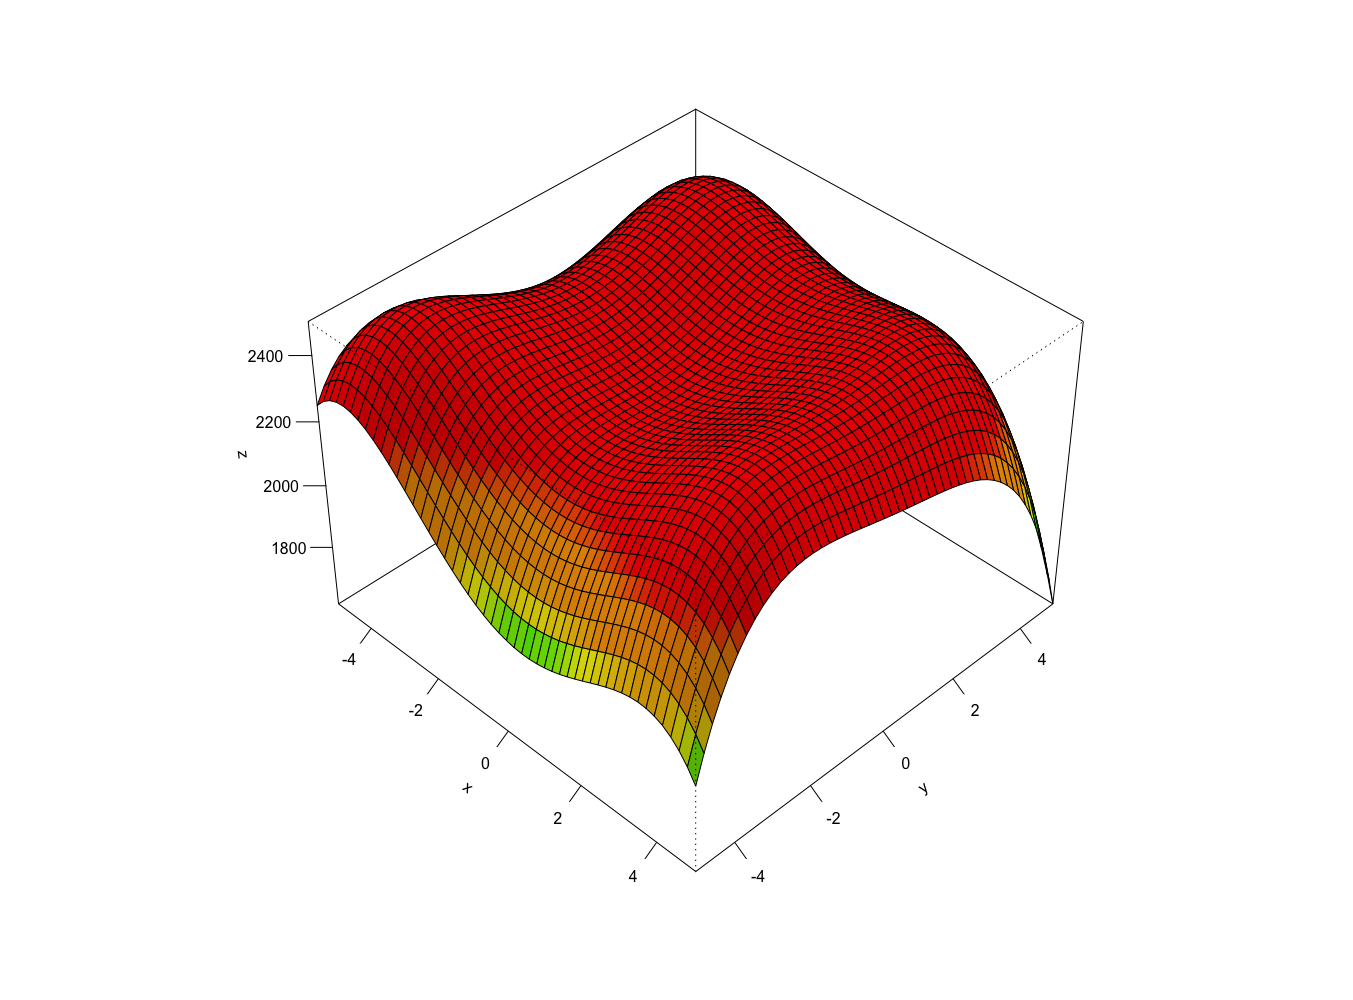
\includegraphics[width=1.7in]{modifiedHimmelblau}} \\
		Sphere & $f(x, y) = -(x^2 + y^2) + 3560$ &$x, y \in [-10;+10]$ & $3560$ & \parbox[c]{1em}{
			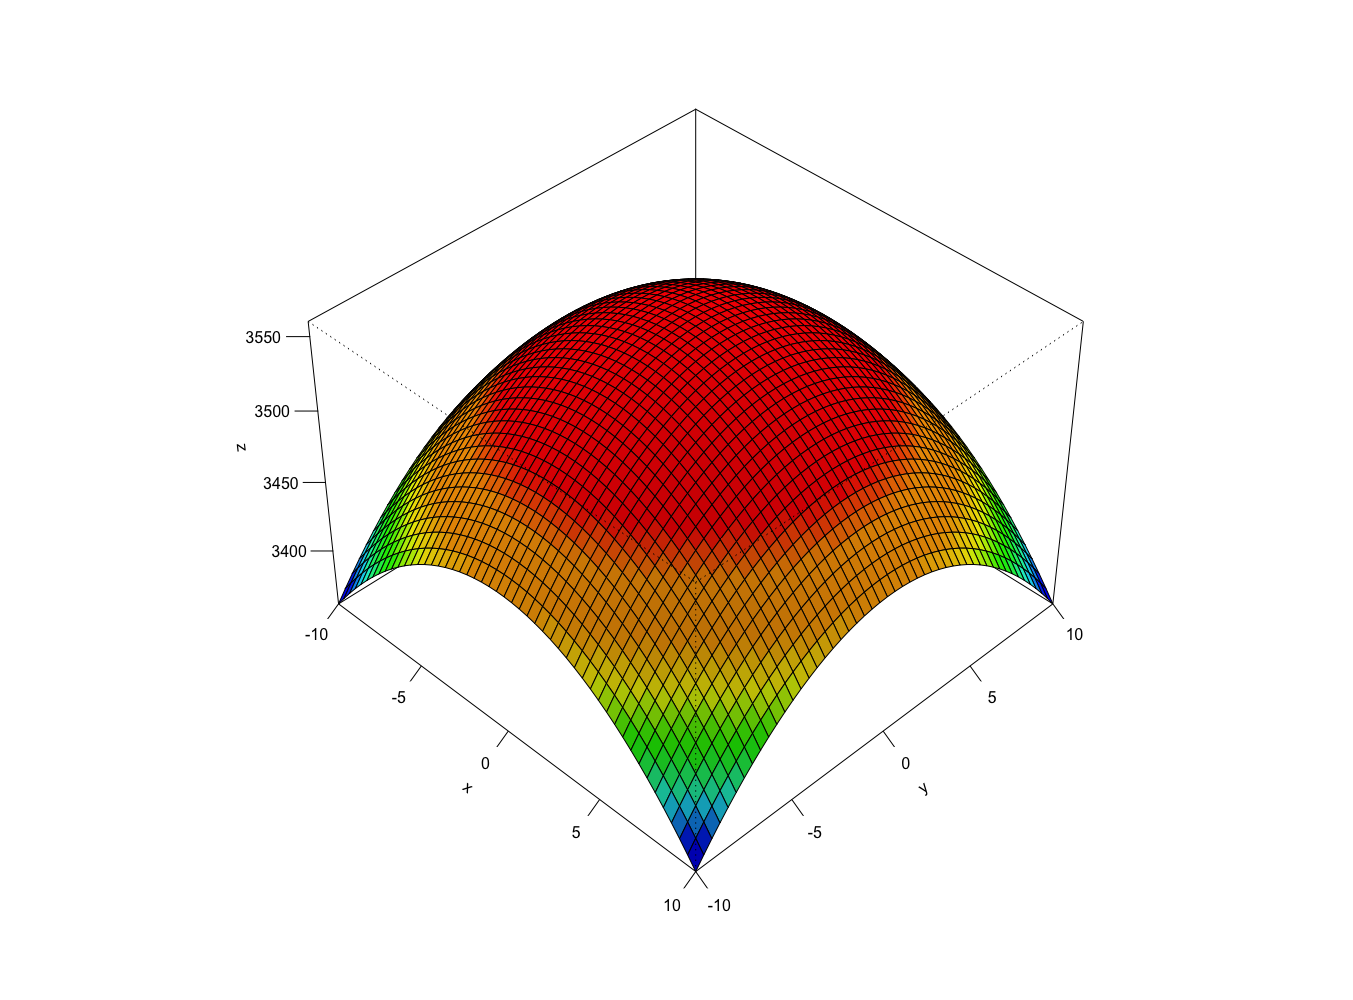
\includegraphics[width=1.7in]{customizedParaboloid}} \\
		Beale & \vtop{\hbox{\strut $f(x, y) = - ((1.5 - x + xy)^2 + ) $}\hbox{\strut $+ (2.25-x+xy^2)^2 + $}\hbox{\strut $+ (2.625 -x+xy^3)^2) + 2000 $}} &$x, y \in [-3;3]$ & $1000$ & \parbox[c]{1em}{
			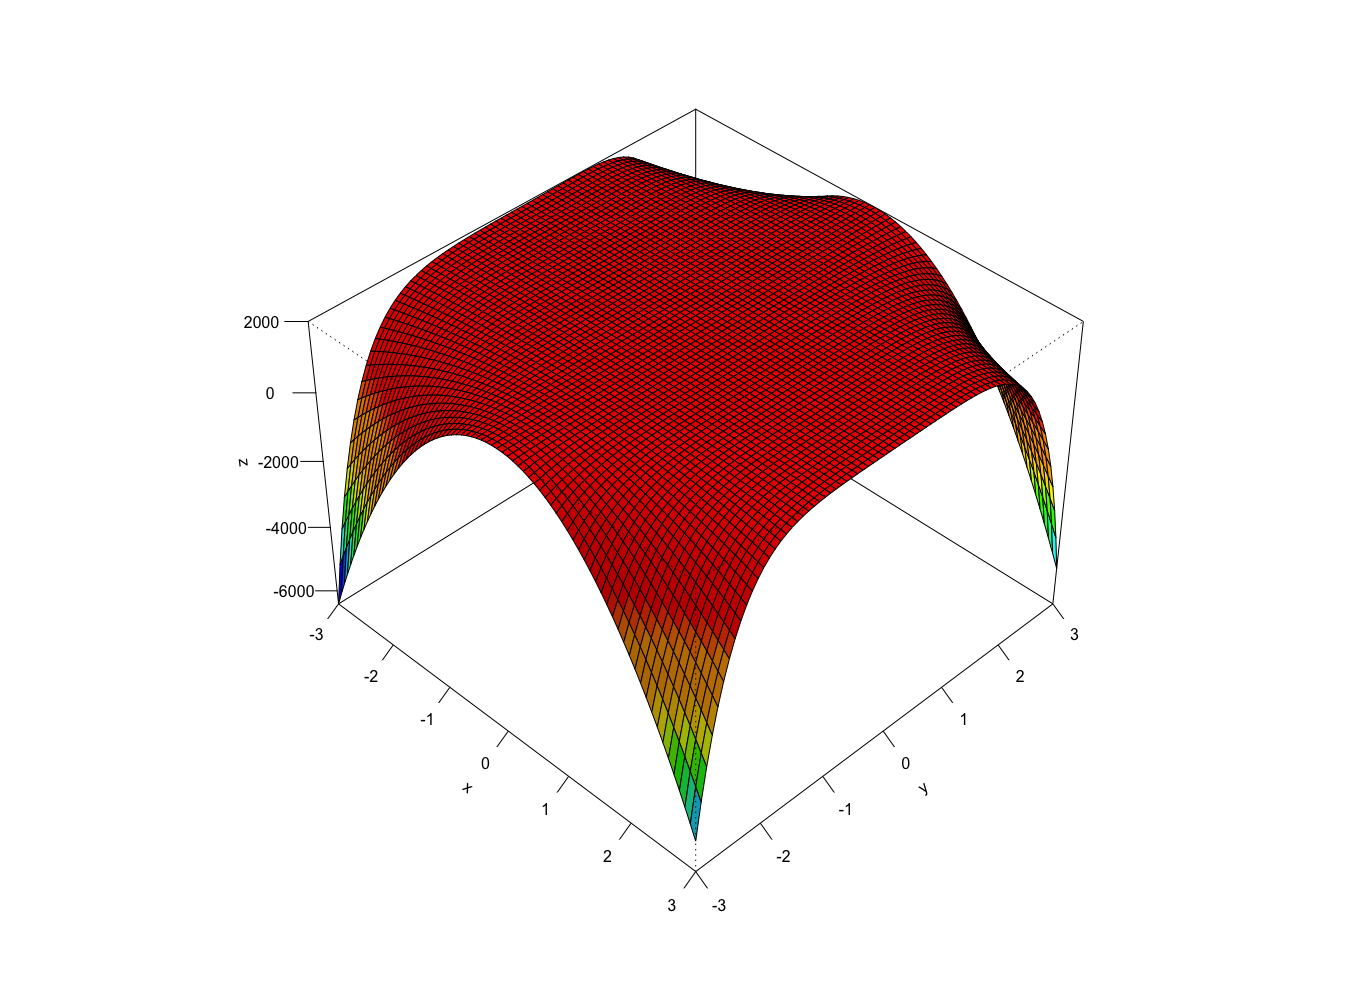
\includegraphics[width=1.7in]{customizedBeale}} \\
		Styblinski-Tang & \vtop{\hbox{\strut $f(x, y) = -((x^4 - 16 * x^2 + 5 * x) + $}\hbox{\strut $(y^4 - 16 * y^2 + 5 * y)) + 5000$}} &$x, y \in [-5;+5]$ & $5156.6638$ & \parbox[c]{1em}{
			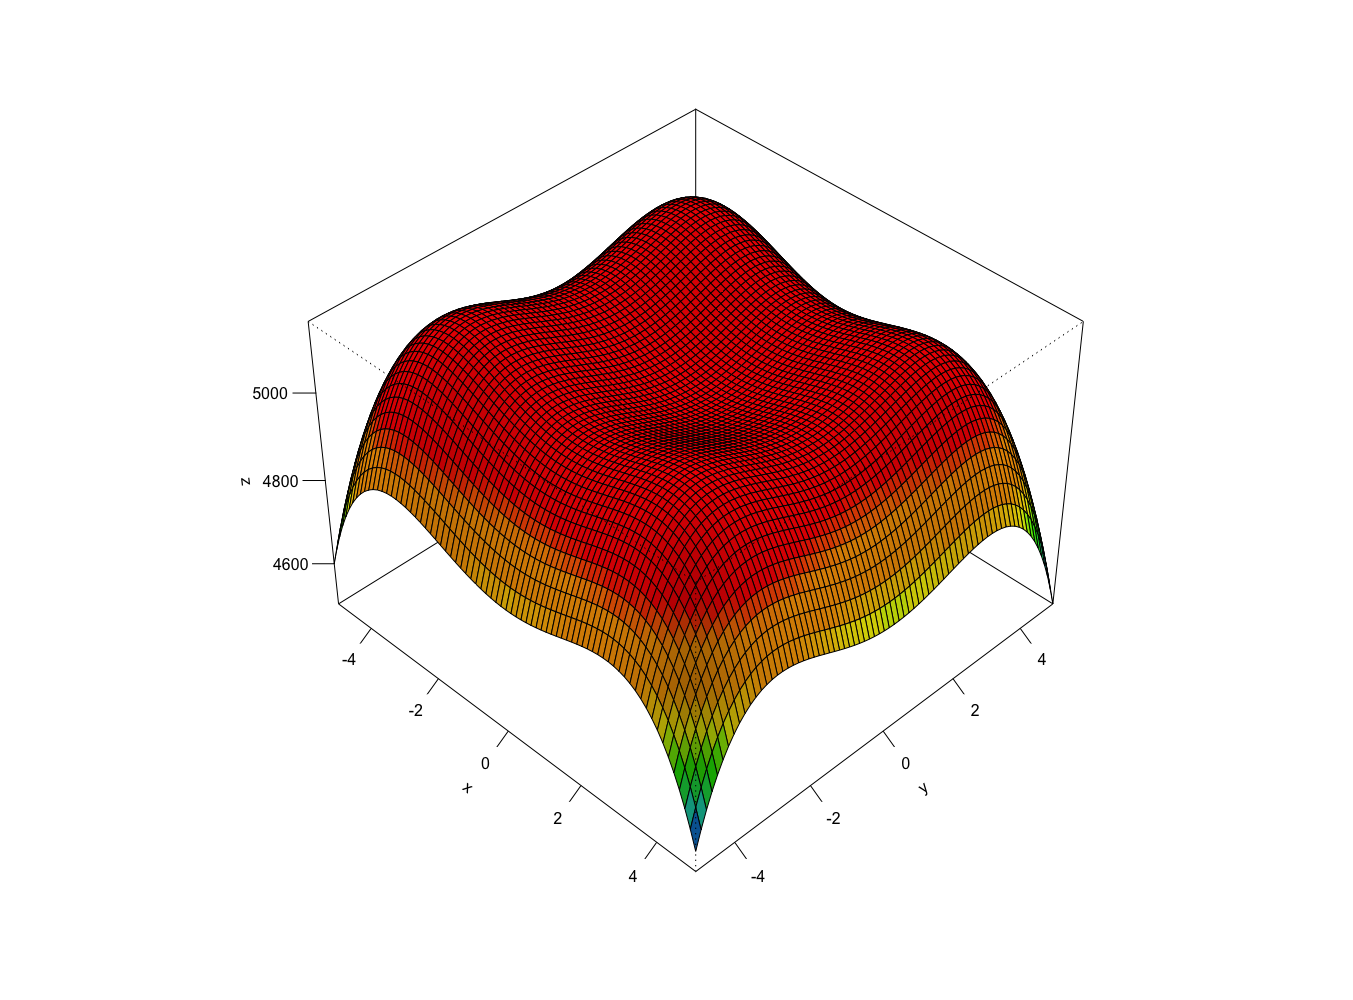
\includegraphics[width=1.7in]{customizedStyblinski}} \\
		\hline
	\end{tabular}
\end{sidewaystable}

\pagebreak

\paragraph{Algorithm Configuration} The RL algorithm employed in the described tests is the {\tt SARSA($\lambda$)} algorithm. Two different configurations are chosen to conduct tests. Both of them are summarized in the following table.

\begin{table} [h!]
	\centering	
	\begin{tabular}{|c|c|c|c|c|c|c|}
		\hline 
		& $\lambda$  & $\epsilon$ & qInit & Learning Rate  & Episodes  & Epochs \\ 
		\hline Configuration $1$
		& $0.1$ & $0.1$ & $0$ & $1$  & $150$ & $100$  \\ 
		\hline Configuration $2$
		& $0.1$ & $0.1$ & $5$ & $1$  & $150$ & $100$  \\ 
		\hline
	\end{tabular} 
\end{table}

In both configurations we used a low $\lambda$ value. The reason is simple. Typically we should use lower learning rates when we have a higher value of $\lambda$. However, in this case, we decide to use the highest possible learning rate. The logical consequence to this choice is to decrease the $\lambda$ value. \\

Also the $\epsilon$ value is equal in both configurations. An $\epsilon$ value equals to $0.1$ means that $90\%$ of selected actions depends on the history, whereas the remaining $10\%$ represent a random choice having absolutely no relations with the previous history. \\ 

The number of episodes and epochs is the same for both configurations. Our goal is to compare human optimization performances with {\tt SARSA($\lambda$)} ones in a context of uncertainty. Assuming that each try has an higher cost, the number of possible tries must be as low as possible assuring, at the same time, a reasonable training space. Note that in addition to training episodes we also have a greedy one. In this case the $\epsilon$ value and the \textit{learning rate} parameter are equals to $0$. Instead, the number of epochs is still the same.  \\

The only difference between the two configurations is the value of the \textit{qInit}. Since SARSA is an iterative algorithm, it implicitly assumes an initial condition before the first update occurs. Initial action values can be used as a simple way of encouraging exploration. Setting the \textit{qInit} to a value higher than $0$ we introduce a sort of \textit{optimism}. This optimism encourages action-value methods to explore. Whichever actions are initially selected, the reward is less than the starting estimates; the learner switches to other actions, being "disappointed" with the rewards it is receiving. The result is that all actions are tried several times before the value estimates converge. We call this technique for encouraging exploration \textit{optimistic initial values}. We regard it as a simple trick that can be quite effective on stationary problems, but it is far from being a generally useful approach to encouraging exploration. For example, it is not well suited to non-stationary problems because its drive for exploration is inherently temporary. If the task changes, creating a renewed need for exploration, this method cannot help. Indeed, any method that focuses on the initial state in any special way is unlikely to help with the general non-stationary case. The beginning of time occurs only once, and thus we should not focus on it too much. This criticism applies as well to the sample-average methods, which also treat the beginning of time as a special event, averaging all subsequent rewards with equal weights. Nevertheless, all of these methods are very simple, and one of them or some simple combination of them is often adequate in practice ~\cite{SuttonBarto}.

\section{Human Case}

The test conducted on humans affects a cross-section of thirty people. In the selection process of test subjects we considered the following three parameters with corresponding bounds :

\begin{itemize}
	\item \textbf{Sex} $\in \{Male, Female\}$
	\item \textbf{Age} $\in [4, 52]$
	\item \textbf{Calculus Knowledge} $\in \{Null, Basic, Advanced\}$ 
\end{itemize}  

Each of the test subjects was placed in front of a personal computer. The following rules have been proposed for individuals over the age of seven:

	
\begin{itemize}
	\item \textit{You will be offered four different levels}.
	\item \textit{The first three levels will need to be repeated three times}.
	\item \textit{The last level can be executed only once}.
	\item \textit{Look carefully at the legend before starting the experiment}.
	\item \textit{At each click you will receive a score with a colour associated with it}.
	\item \textit{The goal is to make as many points as possible with 15 clicks available for each game}.
	\item \textit{No further explanation will be provided}.
\end{itemize}


After that a chromatic scale indicating how positive the reward was for each click was proposed.

\begin{figure}[h!]
	\centering
	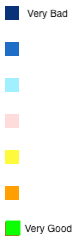
\includegraphics{scala.png}
	\caption{Chromatic Scale.}
	\label{fig:Cromatic Scale}
\end{figure}

A white screen (with a specific hidden function) of $600 \times 600$ pixels with which to interact according to the rules previously listed was finally proposed . For those under the age of seven the selected approach was different. The rules have been explained to them verbally. At each interaction with the environment, in addition to the colour, they were verbally encouraged or discouraged.








